\documentclass[hyperref={pdfpagemode=FullScreen},aspectratio=169]{beamer}
\usetheme[background=dark, numbering=none]{metropolis} % Use metropolis theme 
\usepackage{graphicx} % used for inserting images 
\usepackage{transparent} % used for modifying the opacity of images 
%\usepackage{listings} % used for inserting code 
\usepackage{mathtools}
\usepackage{caption}
\usepackage{color}
\usepackage{amsmath}
\usepackage{listings}
\usepackage{tikz}

% Colors
\definecolor{mDarkBlue}{HTML}{23537F} % m before color stands for monochromatic
\definecolor{mLightBlue}{HTML}{93CCFF}
\definecolor{lightPurple}{HTML}{AA84FD}
\definecolor{purple}{HTML}{8228FA}
\definecolor{magenta}{HTML}{871F61}
\definecolor{lightGreen}{HTML}{5B9E37}

% Alternate Colors 
\definecolor{altSkyBlue}{HTML}{B0E3FF}  
\definecolor{altBlue}{HTML}{266080}
\definecolor{altLightBlue}{HTML}{63D3FF}
\definecolor{white}{HTML}{FFFFFF}
\definecolor{altPurple}{HTML}{5508A6}
\definecolor{altDarkBlue}{HTML}{012340}

% Setting Colors
\setbeamercolor{normal text}{fg=lightPurple, bg=altDarkBlue} % setting the fg and bg colors
\setbeamercolor{title separator}{fg=lightPurple}

\metroset{sectionpage=simple}

\title{\textcolor{lightPurple}{\huge{Introduction to Programming}}}
\date{\large{\today}}
\author{\large{Alexander Hom}}
\institute{\large{Association for Computing Machinery (ACM)}}

\lstset{  %changes the font for lstlisting
  basicstyle=\fontfamily{pxtt}\selectfont,
  keywordstyle=\color{lightGreen},
  showstringspaces=false,
  mathescape
}

\begin{document}
  
  {
  \usebackgroundtemplate{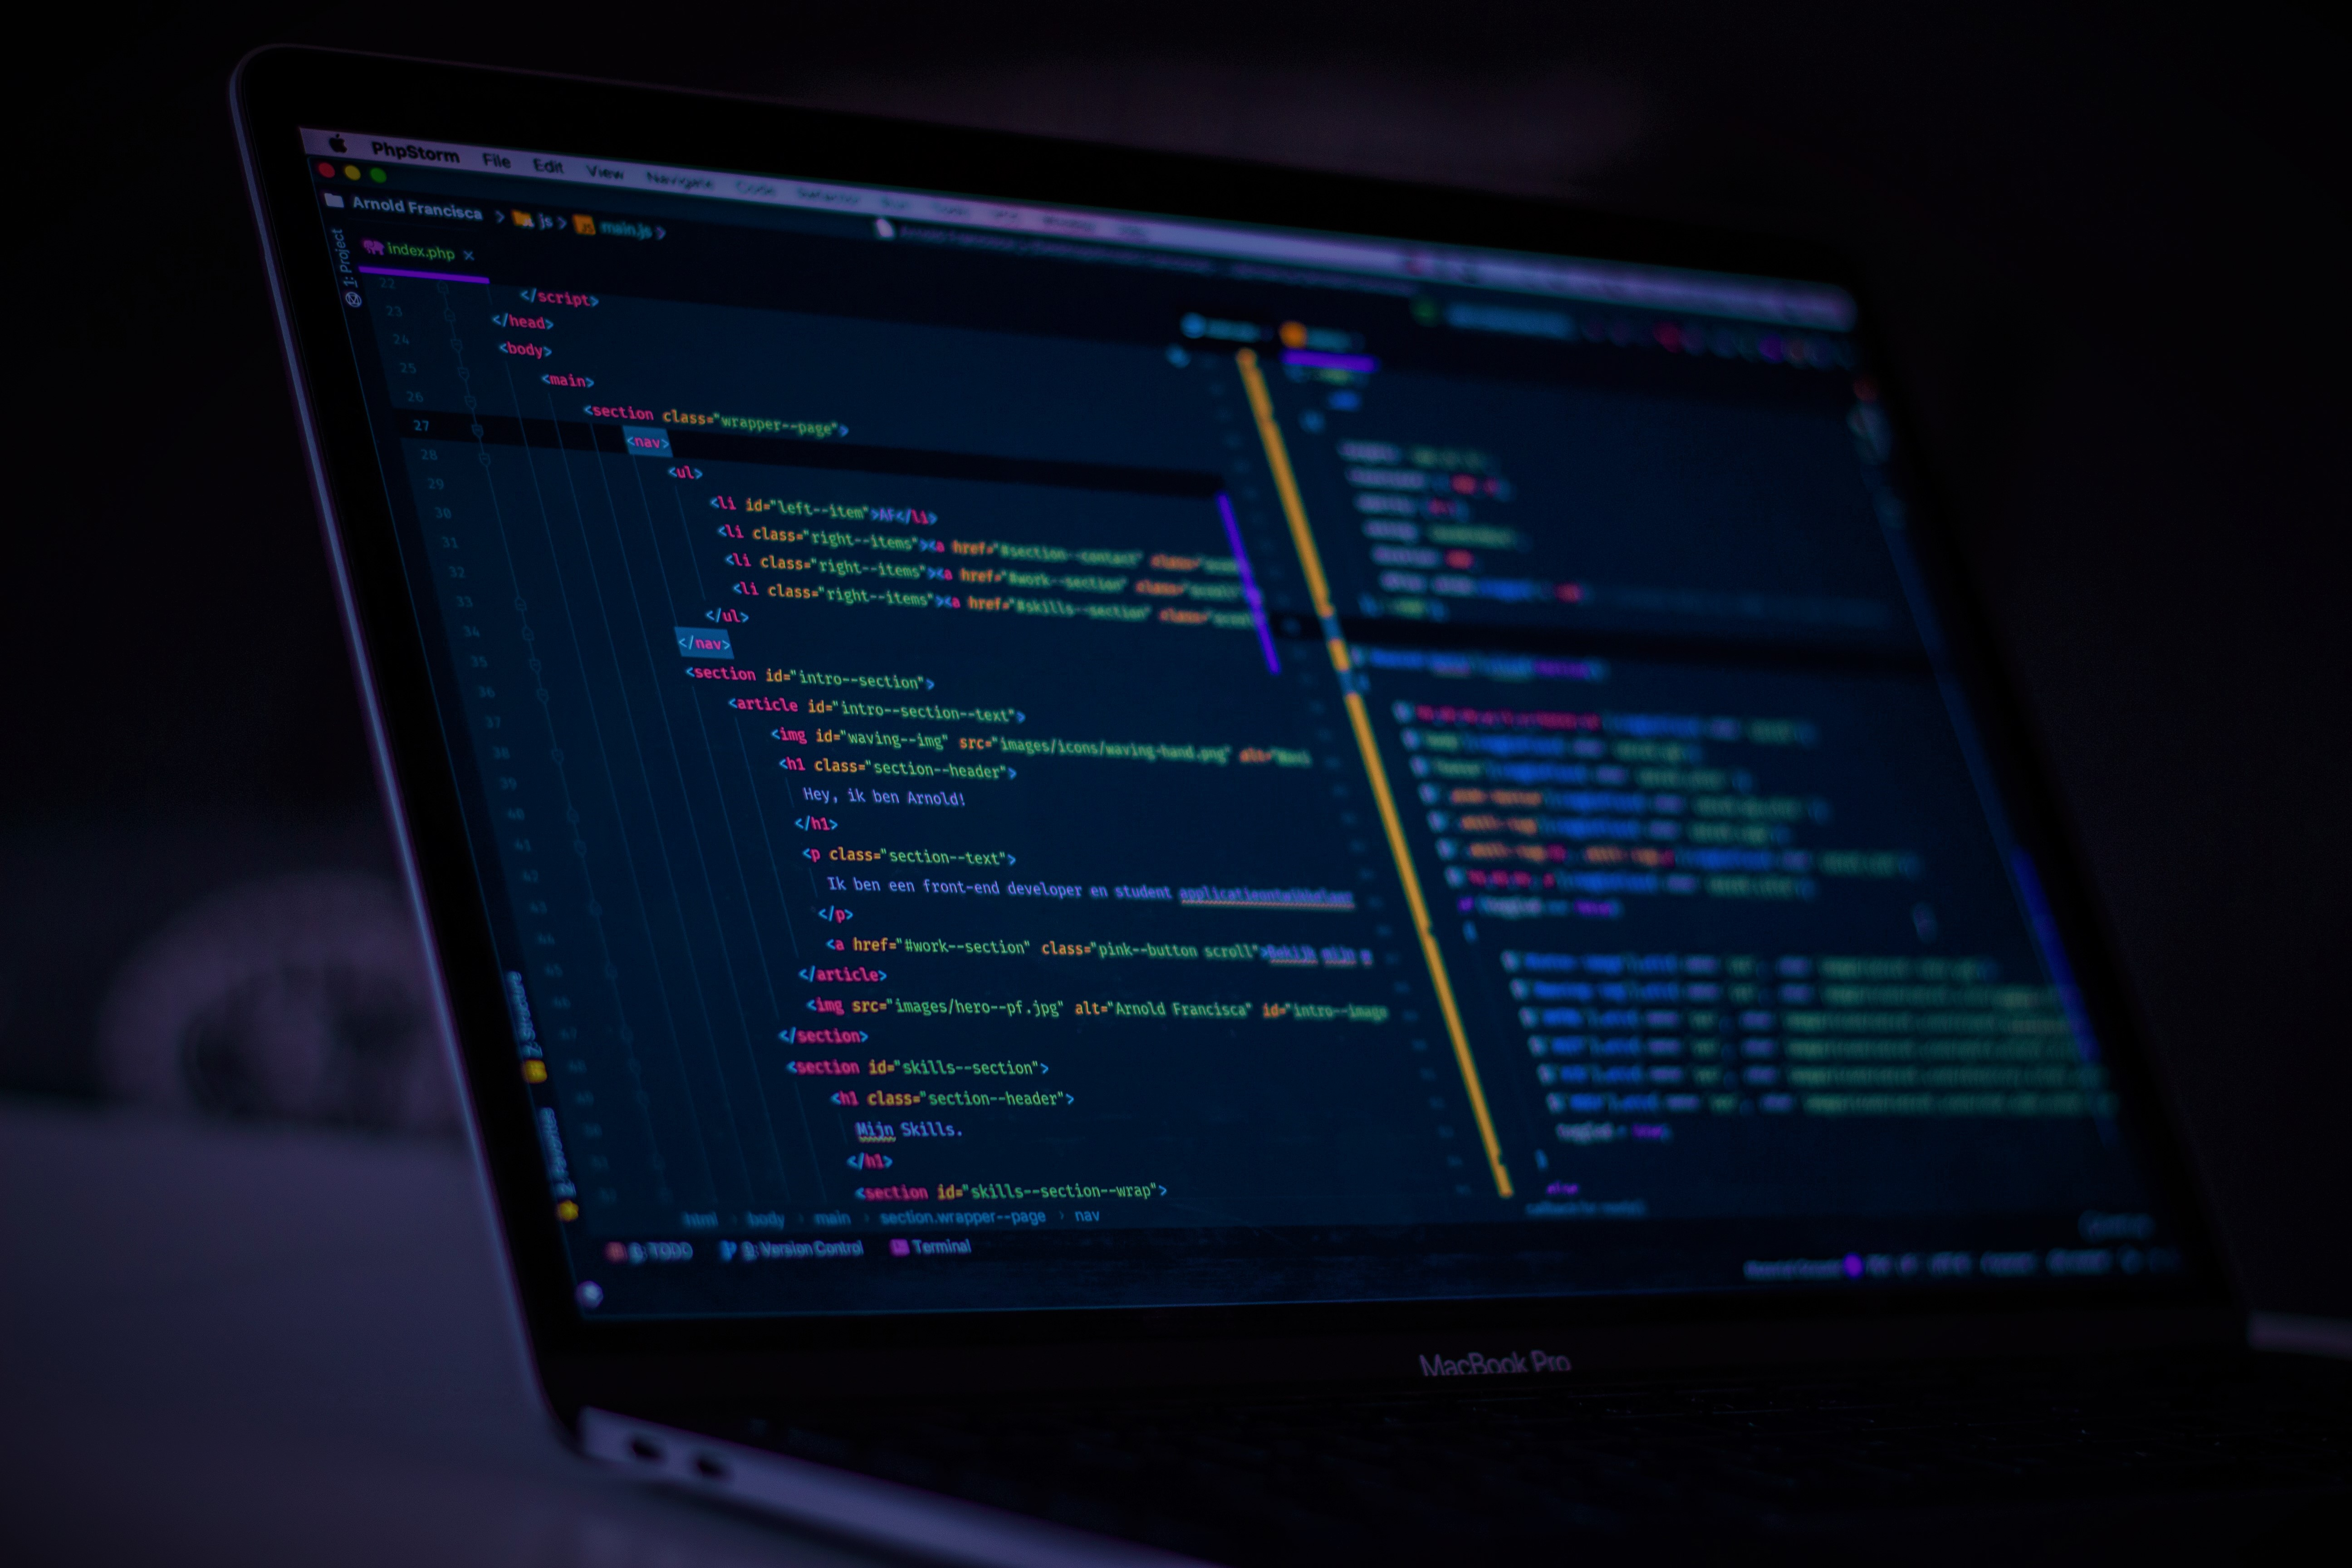
\includegraphics[width=\paperwidth, height=\paperheight]{./imgs/codingImageNineEdited.jpg}}
  \maketitle
  }
  
  \section{\Huge{Introduction}}
  
  \begin{frame}{What is Programming?}
    Today, computers are very smart and powerful, but we often want them to do a specific task that they might not be able to perform on their own. That is where \textcolor{lightGreen}{programming} comes in. Programming allows us to \textit{\textcolor{lightGreen}{talk}} with a computer and let it know what we want it to do. 
  \end{frame}
  
  \begin{frame}{How does Programming Work?}
    Programming sounds \textit{\textcolor{lightGreen}{interesting}}...but how do we do it?\\
    \vspace{0.5cm}
    In order for us to communicate with the computer, we need to use a \textcolor{lightGreen}{language} that both we and the computer can understand. This language takes the form of \textcolor{lightGreen}{code}. 
  \end{frame}
  
  \begin{frame}{Code Example}
    \begin{center}
      \texttt{\textcolor{lightGreen}{print}("Hello, Class!")} $\xrightarrow{\text{\textcolor{lightGreen}{translates into}}}$ Hello, Class!
    \end{center}
  \end{frame}
  
  \begin{frame}{Code Editor}
    \begin{figure}
      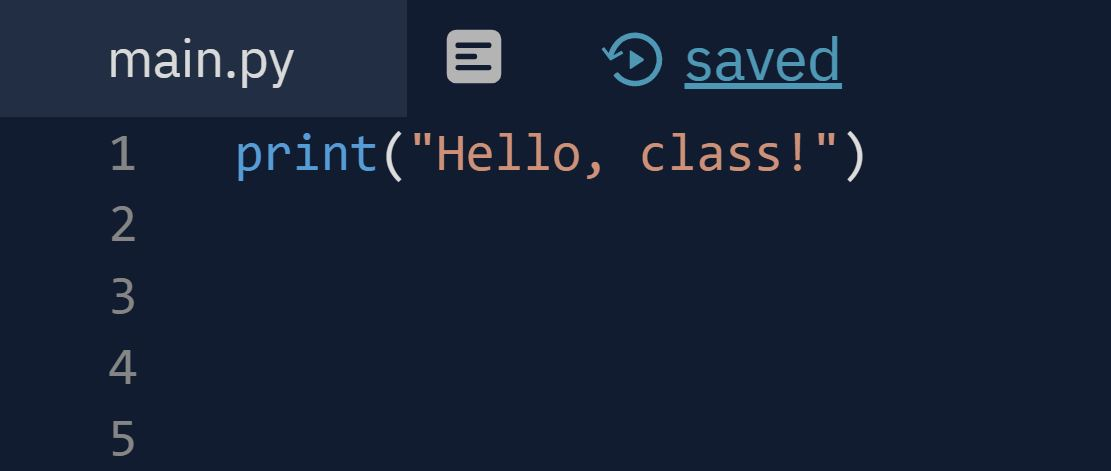
\includegraphics[scale=0.35]{./imgs/helloClassCode.jpg}
      {\caption*{Code is written into the \textcolor{lightGreen}{code editor}}}
    \end{figure}
  \end{frame}
  
  \begin{frame}{Code Output}
    \begin{figure}
      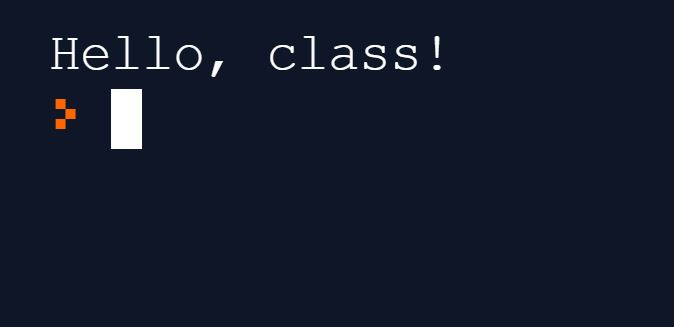
\includegraphics[scale=0.5]{./imgs/helloClassConsoleOutput.jpg}
      {\caption*{The result of our code is displayed in the \textcolor{lightGreen}{console}}} 
    \end{figure}
  \end{frame}
  
  \begin{frame}{Cool Programming Applications}
    Even though we might not see them directly (since code is hidden behind the scenes), the applications of programming can be found everywhere. Some examples include: 
    \begin{itemize}
      \item The apps on our smartphones and computers. 
      \item Websites.
      \item Computers. 
      \item Even this presentation.
      
    \end{itemize}
  \end{frame}
  
  \begin{frame}{What are We Learning Today?}
    Today, we are going to be learning the basics of a programming language called \textcolor{lightGreen}{Python}. We are going to be writing our code in an online coding environment, which makes it easy for us to run and see the results of our code.
  \end{frame}
  
  \begin{frame}{What is Python?}
  Python is a popular programming language and one of the best first languages to learn. It is very approachable to beginners compared to other languages because Python code is read like English sentences and has a simpler syntax (guideline that the code needs to follow).
  
  \end{frame}
  
  \section{\Huge{Activities}}
  
  \begin{frame}{Getting Started} 
    Before we start writing Python code, let's get familiar with the environment with which we are coding on. 
  \end{frame}
  
  \begin{frame}{The Coding Environment}
  \begin{center}
    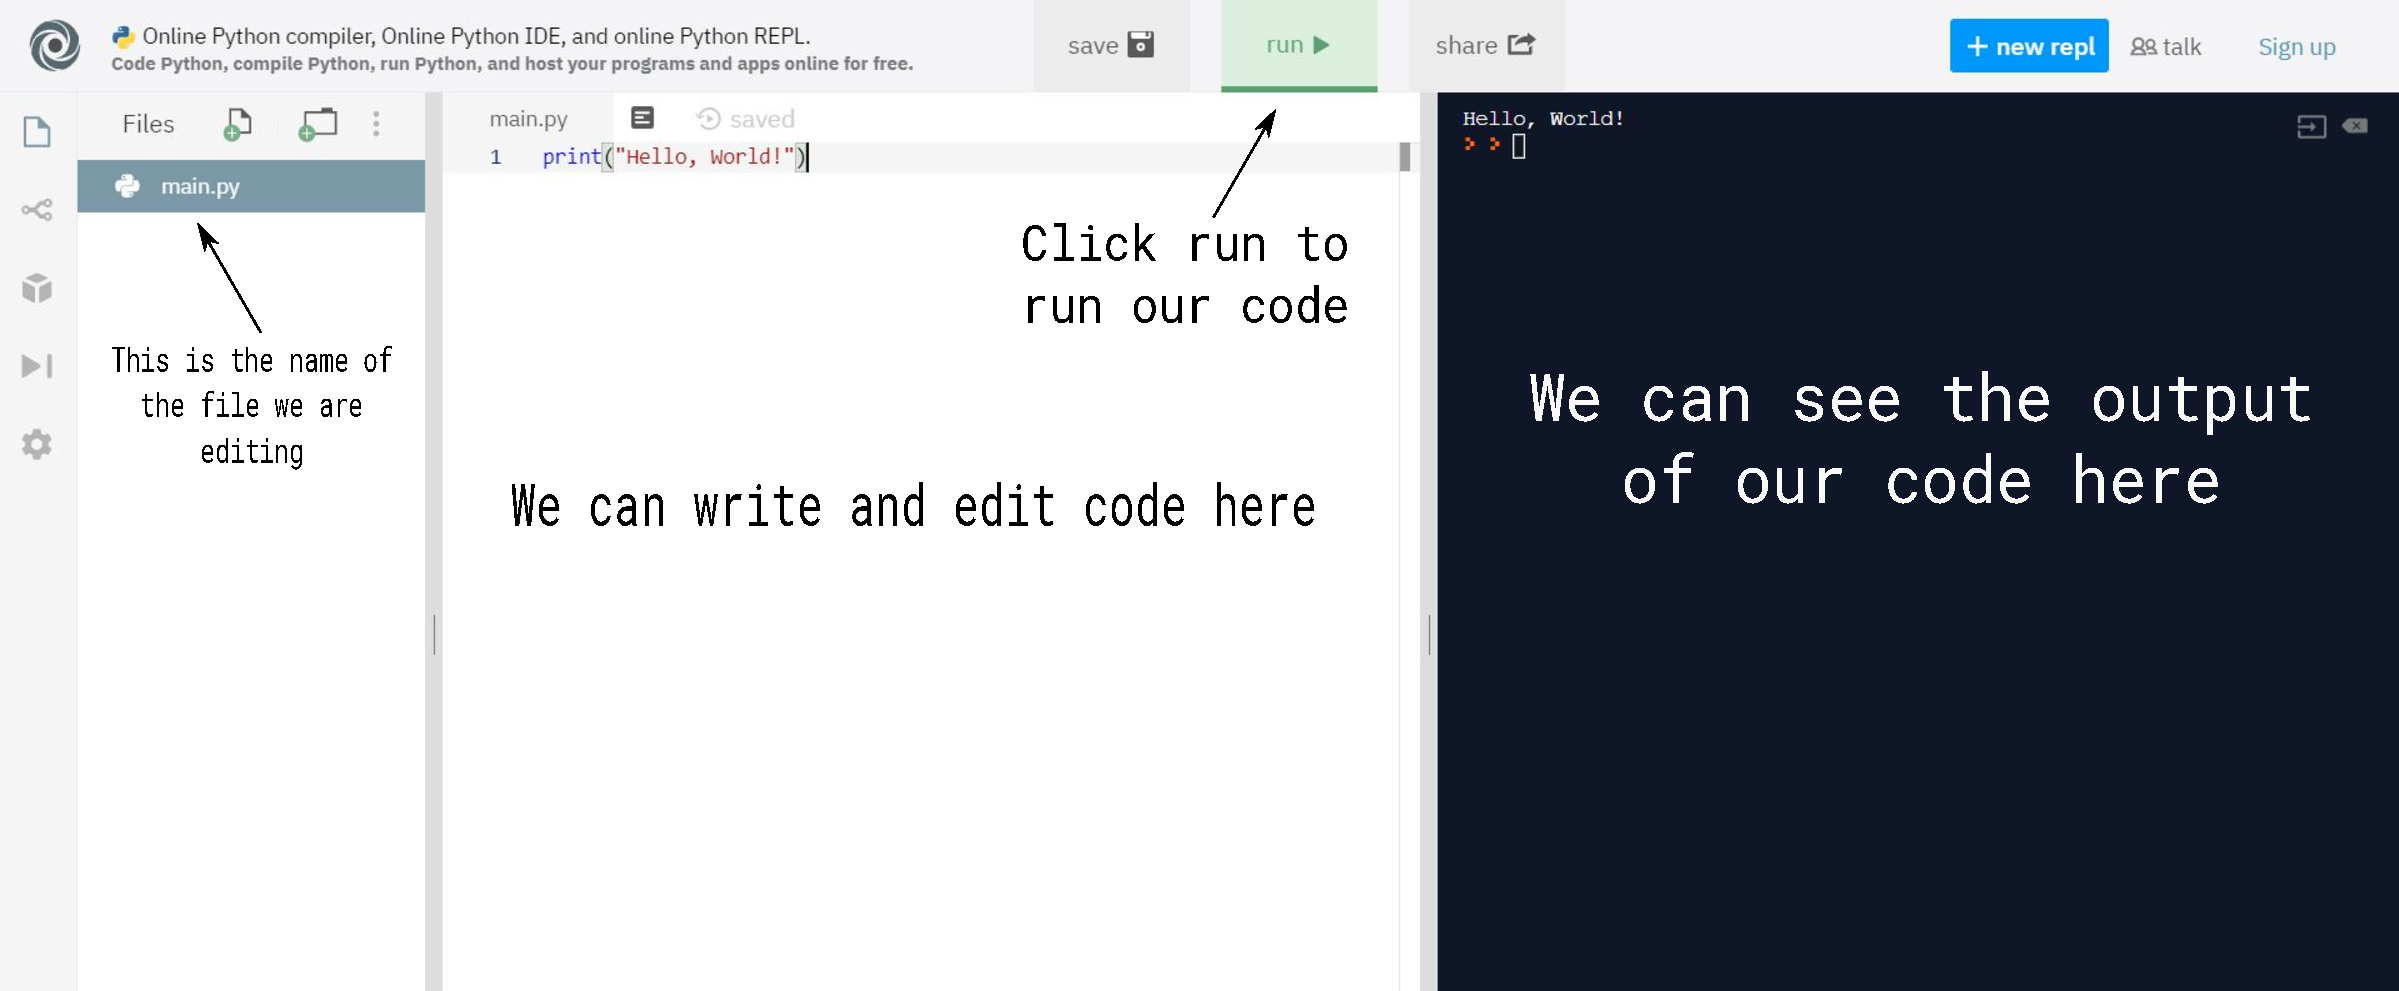
\includegraphics[scale=0.35]{imgs/codeEditor.pdf}
  \end{center}
  \end{frame}
  
  \begin{frame}{Activity 1: Hello World Program}
    Let's start off the coding activities by coding the classic \textit{\textcolor{lightGreen}{Hello World}} program. 
  \end{frame}

  \begin{frame}{Activity 2: Print Statements}
    \begin{figure}
      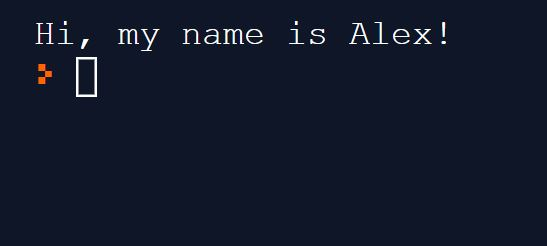
\includegraphics[scale=0.75]{./imgs/activityTwoConsoleOutput.jpg}
      \caption*{Let's try modifying the code so that it prints something else, like your name for instance.}  
    \end{figure}
  \end{frame}

  \begin{frame}{Introduction to Python Grammar Rules (Syntax)}
    Just like in English, there is a gramatical structure that we have to follow when programming in Python and other languages. This structure is called the code's \textcolor{lightGreen}{syntax}. The syntax for Python's \textcolor{lightGreen}{\texttt{print}} function goes like this:  

    \bigskip
    \begin{center}
      $\underbrace{\textcolor{lightGreen}{\texttt{print}}}_{\textcolor{lightGreen}{\text{Action}}}$ ($\underbrace{\texttt{"Hi, my name is Alex!"}}_{\textcolor{lightGreen}{\text{Object that the action is being done on}}}$)
    \end{center}

    \bigskip
    
    There are many other gramatical rules in Python that programmers must follow, which I will introduce later on. 
  \end{frame}

  \begin{frame}{Data Types}
    In the previous two activities, we printed out words. However, we can print out other types of data as well. Here are some \textit{\textcolor{lightGreen}{data types}} that you will encounter in Python and other programming languages: 

    \begin{enumerate}
      \item \textcolor{lightGreen}{\texttt{string}} $\rightarrow$ Words/Phrases/Sentences (i.e., "Hello", "I am a string", \ldots) 
      \item \textcolor{lightGreen}{\texttt{char}} $\rightarrow$ Characters (i.e., 'A', 'B', 'C', \ldots)
      \item \textcolor{lightGreen}{\texttt{int}} $\rightarrow$ Non-decimal numbers (integers) (can be positive or negative)
      \item \textcolor{lightGreen}{\texttt{double}} $\rightarrow$ Decimal numbers (can be positive or negative) 
      \item \textcolor{lightGreen}{\texttt{bool}} $\rightarrow$ True (1) or false (0)
    \end{enumerate}
  \end{frame}

  \begin{frame}{Performing Math Operations}
    So far, we've printed \texttt{\textcolor{lightGreen}{string}}s to the console, but we can also print out other data types, such as numbers (\textcolor{lightGreen}{\texttt{int}} and \textcolor{lightGreen}{\texttt{double}}). One of the nice things about Python is that we can perform math operations on \texttt{\textcolor{lightGreen}{int}}s and \texttt{\textcolor{lightGreen}{double}}s and print out the results to the console:  
 
    \begin{center}
      Addition: \textcolor{lightGreen}{\texttt{print}}\texttt{(5 \textcolor{lightGreen}{+} 10)} $\rightarrow$ Output: 15\\
      Subtraction: \textcolor{lightGreen}{\texttt{print}}\texttt{(8.0 \textcolor{lightGreen}{-} 2.0)} $\rightarrow$ Output: 6.0\\
      Multiplication: \textcolor{lightGreen}{\texttt{print}}\texttt{(17 \textcolor{lightGreen}{*} 3)} $\rightarrow$ Output: 51\\
      Division: \textcolor{lightGreen}{\texttt{print}}\texttt{(30.0 \textcolor{lightGreen}{\slash} 2.0)} $\rightarrow$ Output: 15.0
    \end{center}
  \end{frame}

  \begin{frame}{Activity 3: Printing Numbers}
    Pick two random numbers (for instance, 288 and 97): 
    \begin{enumerate}
      \item Print out the sum of the two numbers
      \item Print out the product of the two numbers
    \end{enumerate}
  \end{frame}

  \begin{frame}{Introduction to Variables}
    We just printed out the sum and product of two numbers. But, what if we want to save the results and use them later on? That's where \textcolor{lightGreen}{variables} come into play. 

    \bigskip
    \textcolor{lightGreen}{Variables} are \textcolor{lightGreen}{\textit{names}} that we can assign to data. For instance, we can add together the numbers 288 and 97 and assign the total number to the variable \textcolor{lightGreen}{\texttt{total}}.

    \begin{center}
      {\Large \textcolor{lightGreen}{\texttt{total}} \texttt{= 288 + 97}}
    \end{center}
  \end{frame}

  \begin{frame}{Rules of Variables}
    To use variables in our code, we have to first introduce them to the computer, otherwise the computer won't know what the variable is: 

    \medskip
    Introducing the variables:
    \begin{itemize}
      \item \textcolor{lightGreen}{\texttt{product}} \texttt{= 56 * 25} 
      
      % $\rightarrow$ The result of 56 * 25 is assigned to the variable \textcolor{lightGreen}{\texttt{product}}
      \item \textcolor{lightGreen}{\texttt{name}} \texttt{= "Alex"} 
      
      % $\rightarrow$ The \textcolor{lightGreen}{\texttt{string}} "Alex" is assigned to the variable \textcolor{lightGreen}{\texttt{name}}
    \end{itemize}

    Calling the variables:
    \begin{itemize}
      \item \textcolor{lightGreen}{\texttt{print}}(\textcolor{lightGreen}{\texttt{product}}) $\rightarrow$ Output: \textcolor{lightGreen}{1400}
      \item \textcolor{lightGreen}{\texttt{print}}("My name is" + \textcolor{lightGreen}{\texttt{name}}) $\rightarrow$ Output: My name is \textcolor{lightGreen}{Alex}
    \end{itemize}

  \end{frame}

  \begin{frame}{Activity 4: Variables Practice}
    Let's use what we have learned so far about printing out words and variables to write a program that displays our \textcolor{lightGreen}{name}, our \textcolor{lightGreen}{favorite color}, and our \textcolor{lightGreen}{favorite animal}. 

    \begin{figure}
      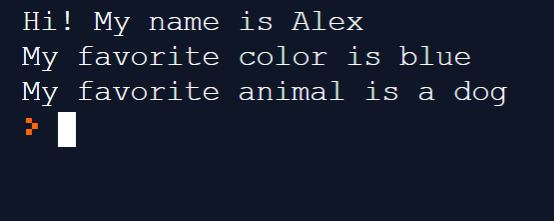
\includegraphics[scale=0.75]{./imgs/activityFourConsoleOutput.jpg}
    \end{figure}

  \end{frame}

  \begin{frame}{Activity 4: Tips and Hints}

    \begin{columns}[c]
      \begin{column}{0.48\textwidth}
        {\small \begin{itemize}
          \item Declare all your variables first
          \item Use simple names for your variables, like \textcolor{lightGreen}{\texttt{favoriteColor}}
          \item Variables can't have spaces. If your variable has more than one word, use:
        
            \begin{itemize}
              \item Camel case $\rightarrow$ \textcolor{lightGreen}{\texttt{favoriteColor}}
              \item Hyphen $\rightarrow$ \textcolor{lightGreen}{\texttt{favorite-color}} 
              \item Underscore $\rightarrow$ \textcolor{lightGreen}{\texttt{favorite\_color}}
            \end{itemize}
        \end{itemize} }
      \end{column}

      \hfill

      \begin{column}{0.48\textwidth}
        \begin{center}
          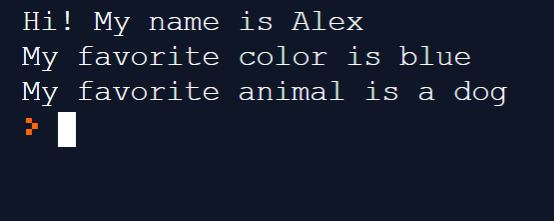
\includegraphics[scale=0.55]{imgs/activityFourConsoleOutput.JPG}
        \end{center}
      \end{column}

    \end{columns}

  \end{frame}

  \begin{frame}{Activity 4: Example Code}
    \begin{center}
      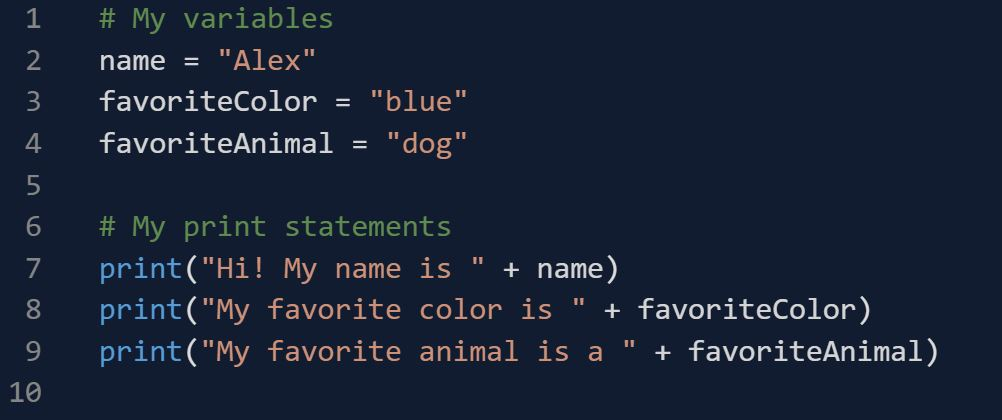
\includegraphics[scale=0.65]{./imgs/activityFourCode.jpg}
    \end{center}
  \end{frame}

  \begin{frame}{Adding Logic to our Code}
    So far, our programs have been one-dimensional, meaning that they run every line of code and perform every action. But what if we want to run certain lines depending on the circumstance, which can change. For example, we have a program that prints the days of the week: 

    \bigskip

    \begin{columns}[c]
      \begin{column}{0.03\textwidth}
      \end{column}
      \begin{column}{0.45\textwidth}
        \begin{figure}
          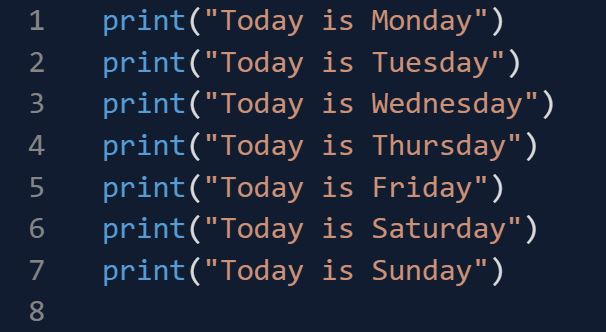
\includegraphics[scale=0.45]{./imgs/logicProgramCode.jpg}
          \caption*{Prints out every day of the week}
        \end{figure}
      \end{column}
  
      \hfill
  
      \begin{column}{0.05\textwidth}
        {\huge $\rightarrow$}
      \end{column}
  
      \hfill
  
      \begin{column}{0.43\textwidth}
        \begin{figure}
          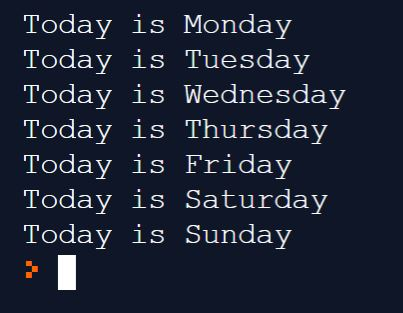
\includegraphics[scale=0.5]{./imgs/logicProgramOutput.jpg}
          \caption*{Only want to print out Saturday}
        \end{figure}
      \end{column}
    \end{columns}
  \end{frame}

  \begin{frame}{Introduction to Conditional Statements}
    Rather than having the program print out all the days of the week, we can have it just print out today, Saturday, with the help of a \textcolor{lightGreen}{conditional statement}.\\

    In English, conditionals are the \textcolor{lightGreen}{ifs} and \textcolor{lightGreen}{elses} that we sometimes use in our conversations: 

    \begin{center}
      \textcolor{lightGreen}{If} it is raining, then I will bring an umbrella. Otherwise (\textcolor{lightGreen}{else}), I won't.\\

      \smallskip
      \textcolor{lightGreen}{If} today is Saturday, then the program will print out Saturday. \textcolor{lightGreen}{Else}, it will print out a different day.
    \end{center}
  \end{frame}

  \begin{frame}[fragile]{The If-Else statement} %[fragile] for slides with code in it
    To add a condition statement in our programs, we can use \textcolor{lightGreen}{if-else} statements. The syntax for \textcolor{lightGreen}{if-else} statments in Python goes like this:
    \begin{center}  
      \begin{tabular}{c}  % Using tabular for centering lstlisting
        \begin{lstlisting}[language=Python]
if (condition_1):
  perform action_1
elif (condition_2):
  perform action_2
else:
  perform action_3
        \end{lstlisting}
      \end{tabular}
    \end{center}

    % \begin{tikzpicture}
      
    % \end{tikzpicture}
  \end{frame}

  \begin{frame}[fragile]{If-Else Example}
    \begin{columns}[c]
      \begin{column}{0.03\textwidth}
        
      \end{column}

      \hfill 

      \begin{column}{0.48\textwidth}
        \begin{lstlisting}[language=Python]
today = "Saturday"

if (today == "Saturday"):
  print("Today is Saturday")
else: 
  print("Today is NOT Saturday")
        \end{lstlisting}
      \end{column}

      \hfill 

      \begin{column}{0.08\textwidth}
        {\huge $\rightarrow$}
      \end{column}

      \hfill

      \begin{column}{0.38\textwidth}
        Today is Saturday
      \end{column}

    \end{columns}
  
  \end{frame}

  \begin{frame}{Activity 5: If-Else Statements Practice}
    Sam is planning on watching a movie tonight, but is unsure of what movie to watch. Let's write a program using \textcolor{lightGreen}{if-else} statements that will help Sam decide on a movie. 
  \end{frame}

  \begin{frame}{Activity 5: Outline of Movie-Choosing Program}
    \begin{itemize}
      \item Sam can choose from five genres of movies (action, romance, comedy, science fiction, and random)
      \item The program will list the movie genres and ask Sam to pick from one of the five genres
      \item The program will display a movie based on which genre Sam picked
    \end{itemize}
  \end{frame}

  \begin{frame}{Activity 5: Code}
    \begin{columns}[c]
      \begin{column}{0.45\textwidth}
        \begin{center}
          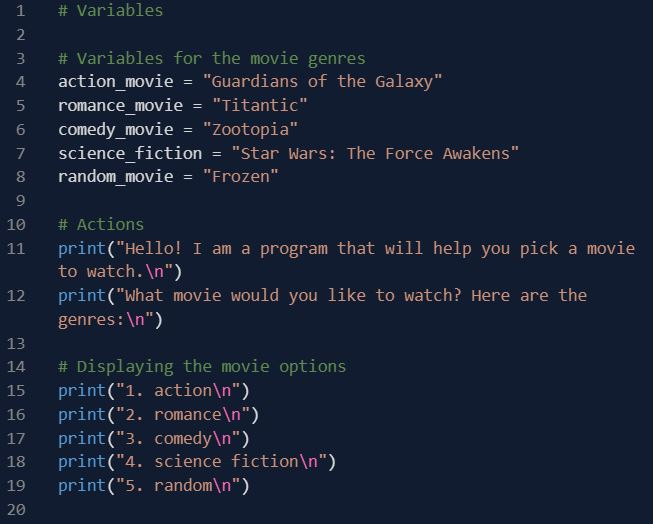
\includegraphics[scale=0.5]{./imgs/activityFiveCodePart1.jpg}
        \end{center}
      \end{column}

      \hfill

      \begin{column}{0.45\textwidth}
        \begin{center}
          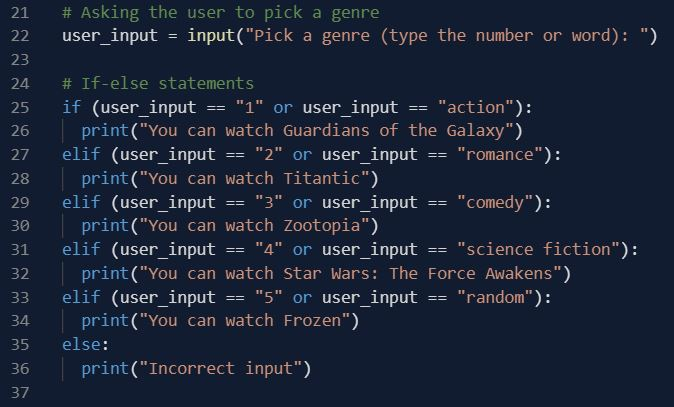
\includegraphics[scale=0.45]{./imgs/activityFiveCodePart2.jpg}
        \end{center}
      \end{column}
    \end{columns}
  \end{frame}

  \begin{frame}{Activity 5 Bonus: Alternate Movie-Choosing Program}
    As a bonus: here's another way of performing the same thing as the previous program, but this time using something called \textcolor{lightGreen}{\texttt{arrays}} and \textcolor{lightGreen}{\texttt{for-loops}} that help make the code more efficient. 
  \end{frame}

  \begin{frame}{Activity 5 Bonus: Code}
    \begin{columns}[c]
      \begin{column}{0.45\textwidth}
        \begin{center}
          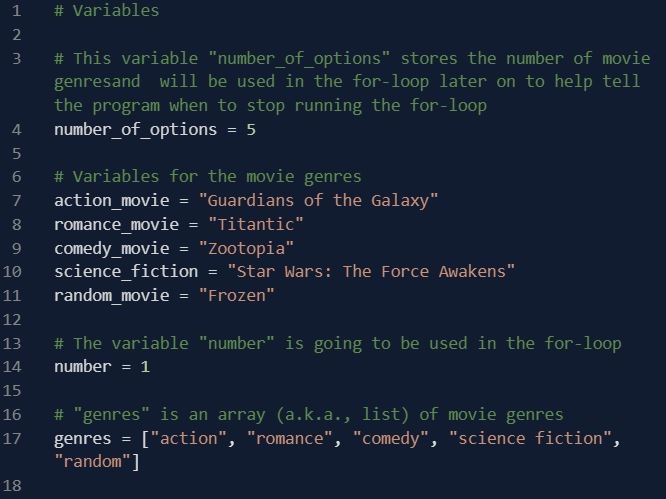
\includegraphics[scale=0.5]{./imgs/activityFiveAlternateCodePart1.jpg}
        \end{center}
      \end{column}

      \hfill 

      \begin{column}{0.45\textwidth}
        \begin{center}
          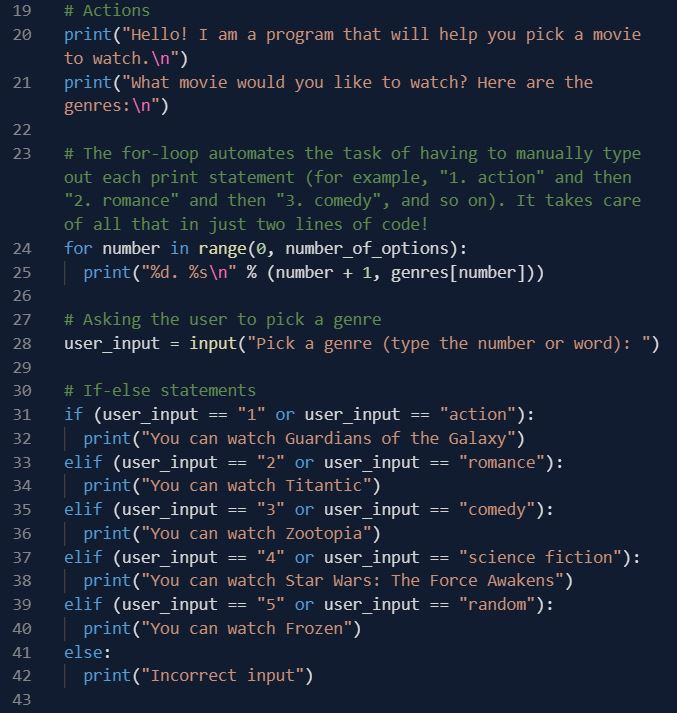
\includegraphics[scale=0.43]{./imgs/activityFiveAlternateCodePart2.jpg}
        \end{center}
      \end{column}
    \end{columns}
  \end{frame}

  \begin{frame}{Activity 5: Output}

    \begin{columns}[c]
      \begin{column}{0.48\textwidth}
        \begin{center}
          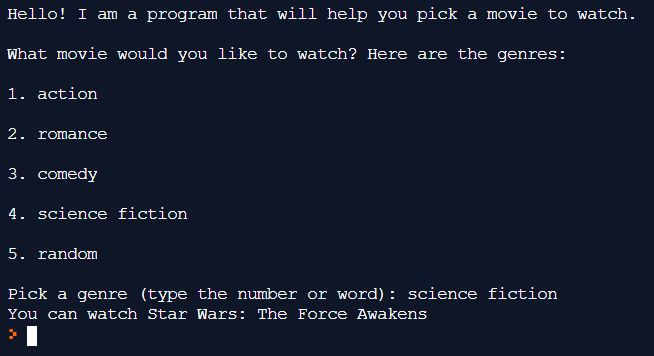
\includegraphics[scale=0.48]{./imgs/activityFiveOutputPart1.jpg}
        \end{center}
      \end{column}

      \hfill

      \begin{column}{0.48\textwidth}
        \begin{center}
          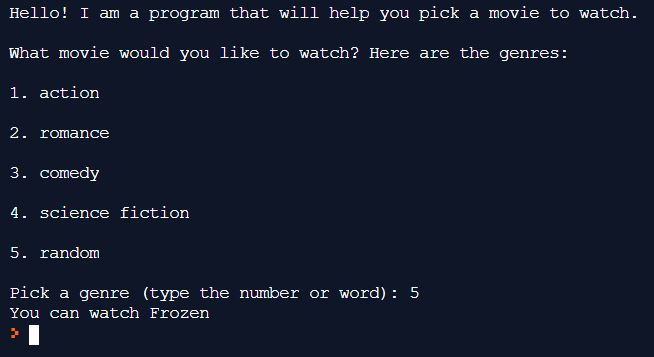
\includegraphics[scale=0.48]{./imgs/activityFiveOutputPart2.jpg}
        \end{center}
      \end{column}
    \end{columns}

    \begin{center}
      Both versions of the program display the same output
    \end{center}
    
  \end{frame}

  \section{\Huge{Wrapping Up}}

  \begin{frame}{Recap of the Workshop}
    In today's workshop we learned:
    \begin{enumerate}
      \item What programming is and some of its real-world applications
      \item How to interact with an online code editor called \textcolor{lightGreen}{repl.it}
      \item How to print words and numbers in Python 
      \item Some grammar rules (syntax) that applies to Python
      \item How to perform math operations using Python 
      \item The basics of variables
      \item How to implement some logic in our code using \textcolor{lightGreen}{if-else} statements
    \end{enumerate}

  \end{frame}

  \section{\Huge{Questions?}}

  \section{\Huge{Thank You!}}
  
\end{document}